% Options for packages loaded elsewhere
\PassOptionsToPackage{unicode}{hyperref}
\PassOptionsToPackage{hyphens}{url}
%
\documentclass[
  12pt,
]{article}
\usepackage{lmodern}
\usepackage{amssymb,amsmath}
\usepackage{ifxetex,ifluatex}
\ifnum 0\ifxetex 1\fi\ifluatex 1\fi=0 % if pdftex
  \usepackage[T1]{fontenc}
  \usepackage[utf8]{inputenc}
  \usepackage{textcomp} % provide euro and other symbols
\else % if luatex or xetex
  \usepackage{unicode-math}
  \defaultfontfeatures{Scale=MatchLowercase}
  \defaultfontfeatures[\rmfamily]{Ligatures=TeX,Scale=1}
  \setmainfont[]{Times New Roman}
\fi
% Use upquote if available, for straight quotes in verbatim environments
\IfFileExists{upquote.sty}{\usepackage{upquote}}{}
\IfFileExists{microtype.sty}{% use microtype if available
  \usepackage[]{microtype}
  \UseMicrotypeSet[protrusion]{basicmath} % disable protrusion for tt fonts
}{}
\makeatletter
\@ifundefined{KOMAClassName}{% if non-KOMA class
  \IfFileExists{parskip.sty}{%
    \usepackage{parskip}
  }{% else
    \setlength{\parindent}{0pt}
    \setlength{\parskip}{6pt plus 2pt minus 1pt}}
}{% if KOMA class
  \KOMAoptions{parskip=half}}
\makeatother
\usepackage{xcolor}
\IfFileExists{xurl.sty}{\usepackage{xurl}}{} % add URL line breaks if available
\IfFileExists{bookmark.sty}{\usepackage{bookmark}}{\usepackage{hyperref}}
\hypersetup{
  pdftitle={Effects of a Defaunation Gradient on Tropical Forest Structure in Ivindo National Park, Gabon},
  pdfauthor={Tashsa Griffiths, Israel Golden, Aubrey Knier, and Mishka Malinowski},
  hidelinks,
  pdfcreator={LaTeX via pandoc}}
\urlstyle{same} % disable monospaced font for URLs
\usepackage[margin=2.54cm]{geometry}
\usepackage{longtable,booktabs}
% Correct order of tables after \paragraph or \subparagraph
\usepackage{etoolbox}
\makeatletter
\patchcmd\longtable{\par}{\if@noskipsec\mbox{}\fi\par}{}{}
\makeatother
% Allow footnotes in longtable head/foot
\IfFileExists{footnotehyper.sty}{\usepackage{footnotehyper}}{\usepackage{footnote}}
\makesavenoteenv{longtable}
\usepackage{graphicx,grffile}
\makeatletter
\def\maxwidth{\ifdim\Gin@nat@width>\linewidth\linewidth\else\Gin@nat@width\fi}
\def\maxheight{\ifdim\Gin@nat@height>\textheight\textheight\else\Gin@nat@height\fi}
\makeatother
% Scale images if necessary, so that they will not overflow the page
% margins by default, and it is still possible to overwrite the defaults
% using explicit options in \includegraphics[width, height, ...]{}
\setkeys{Gin}{width=\maxwidth,height=\maxheight,keepaspectratio}
% Set default figure placement to htbp
\makeatletter
\def\fps@figure{htbp}
\makeatother
\setlength{\emergencystretch}{3em} % prevent overfull lines
\providecommand{\tightlist}{%
  \setlength{\itemsep}{0pt}\setlength{\parskip}{0pt}}
\setcounter{secnumdepth}{5}

\title{Effects of a Defaunation Gradient on Tropical Forest Structure in Ivindo
National Park, Gabon}
\usepackage{etoolbox}
\makeatletter
\providecommand{\subtitle}[1]{% add subtitle to \maketitle
  \apptocmd{\@title}{\par {\large #1 \par}}{}{}
}
\makeatother
\subtitle{\url{https://github.com/israelgolden/GoldenGriffithsKnierMalinowski_ENV872_EDA_FinalProject}}
\author{Tashsa Griffiths, Israel Golden, Aubrey Knier, and Mishka Malinowski}
\date{}

\begin{document}
\maketitle

\newpage
\tableofcontents 
\newpage
\listoftables 
\newpage
\listoffigures 
\newpage

\hypertarget{rationale-and-research-questions}{%
\section{Rationale and Research
Questions}\label{rationale-and-research-questions}}

\newpage

\hypertarget{dataset-information}{%
\section{Dataset Information}\label{dataset-information}}

This dataset if provided by the Pouslen Tropical Ecology Lab here at
Duke. yadda yadda\ldots{}

\ldots briefly explain what the project is / what the data are\ldots{}

The dimensions and variable information of the raw dataset are below:

\begin{verbatim}
## [1] 45681    21
\end{verbatim}

\begin{longtable}[]{@{}llll@{}}
\toprule
\begin{minipage}[b]{0.18\columnwidth}\raggedright
Column name\strut
\end{minipage} & \begin{minipage}[b]{0.35\columnwidth}\raggedright
Description\strut
\end{minipage} & \begin{minipage}[b]{0.18\columnwidth}\raggedright
Unit\strut
\end{minipage} & \begin{minipage}[b]{0.18\columnwidth}\raggedright
Range (if applicable)\strut
\end{minipage}\tabularnewline
\midrule
\endhead
\begin{minipage}[t]{0.18\columnwidth}\raggedright
E\strut
\end{minipage} & \begin{minipage}[t]{0.35\columnwidth}\raggedright
Field expedition season\strut
\end{minipage} & \begin{minipage}[t]{0.18\columnwidth}\raggedright
Season-Year\strut
\end{minipage} & \begin{minipage}[t]{0.18\columnwidth}\raggedright
Winter - Summer 2021\strut
\end{minipage}\tabularnewline
\begin{minipage}[t]{0.18\columnwidth}\raggedright
Data\_entry\strut
\end{minipage} & \begin{minipage}[t]{0.35\columnwidth}\raggedright
Name of individual inputting data to Excel\strut
\end{minipage} & \begin{minipage}[t]{0.18\columnwidth}\raggedright
Name\strut
\end{minipage} & \begin{minipage}[t]{0.18\columnwidth}\raggedright
\strut
\end{minipage}\tabularnewline
\begin{minipage}[t]{0.18\columnwidth}\raggedright
Date..dd.mm.yyyy.\strut
\end{minipage} & \begin{minipage}[t]{0.35\columnwidth}\raggedright
Date of Excel data entry\strut
\end{minipage} & \begin{minipage}[t]{0.18\columnwidth}\raggedright
Date/Month/Year\strut
\end{minipage} & \begin{minipage}[t]{0.18\columnwidth}\raggedright
March 2021 - November 2022\strut
\end{minipage}\tabularnewline
\begin{minipage}[t]{0.18\columnwidth}\raggedright
File\_name\strut
\end{minipage} & \begin{minipage}[t]{0.35\columnwidth}\raggedright
Photo file name of field data sheet\strut
\end{minipage} & \begin{minipage}[t]{0.18\columnwidth}\raggedright
.JPG\strut
\end{minipage} & \begin{minipage}[t]{0.18\columnwidth}\raggedright
\strut
\end{minipage}\tabularnewline
\begin{minipage}[t]{0.18\columnwidth}\raggedright
Date..dd.mm.yyyy..1\strut
\end{minipage} & \begin{minipage}[t]{0.35\columnwidth}\raggedright
Data of field data collection\strut
\end{minipage} & \begin{minipage}[t]{0.18\columnwidth}\raggedright
Date/Month/Year\strut
\end{minipage} & \begin{minipage}[t]{0.18\columnwidth}\raggedright
June - January 2021\strut
\end{minipage}\tabularnewline
\begin{minipage}[t]{0.18\columnwidth}\raggedright
Note\_taker\strut
\end{minipage} & \begin{minipage}[t]{0.35\columnwidth}\raggedright
Name of individual recording field data\strut
\end{minipage} & \begin{minipage}[t]{0.18\columnwidth}\raggedright
Name\strut
\end{minipage} & \begin{minipage}[t]{0.18\columnwidth}\raggedright
\strut
\end{minipage}\tabularnewline
\begin{minipage}[t]{0.18\columnwidth}\raggedright
Project\strut
\end{minipage} & \begin{minipage}[t]{0.35\columnwidth}\raggedright
Defaunated forest (DF) or intact forest (IF) plot\strut
\end{minipage} & \begin{minipage}[t]{0.18\columnwidth}\raggedright
Category\strut
\end{minipage} & \begin{minipage}[t]{0.18\columnwidth}\raggedright
DF or IF\strut
\end{minipage}\tabularnewline
\begin{minipage}[t]{0.18\columnwidth}\raggedright
Plot\strut
\end{minipage} & \begin{minipage}[t]{0.35\columnwidth}\raggedright
Unique plot identification\strut
\end{minipage} & \begin{minipage}[t]{0.18\columnwidth}\raggedright
Category\strut
\end{minipage} & \begin{minipage}[t]{0.18\columnwidth}\raggedright
1A, 1B, 2A, 2B, 3A, 3B, 4A, 4B, 5A, 5B, 6A, 6B\strut
\end{minipage}\tabularnewline
\begin{minipage}[t]{0.18\columnwidth}\raggedright
Grid\strut
\end{minipage} & \begin{minipage}[t]{0.35\columnwidth}\raggedright
Within-plot grid where data were collected\strut
\end{minipage} & \begin{minipage}[t]{0.18\columnwidth}\raggedright
Category\strut
\end{minipage} & \begin{minipage}[t]{0.18\columnwidth}\raggedright
\strut
\end{minipage}\tabularnewline
\begin{minipage}[t]{0.18\columnwidth}\raggedright
TAG\_SUM\strut
\end{minipage} & \begin{minipage}[t]{0.35\columnwidth}\raggedright
The most unique identifier, using plot grid and plant tag\strut
\end{minipage} & \begin{minipage}[t]{0.18\columnwidth}\raggedright
Category\strut
\end{minipage} & \begin{minipage}[t]{0.18\columnwidth}\raggedright
\strut
\end{minipage}\tabularnewline
\begin{minipage}[t]{0.18\columnwidth}\raggedright
Plant\_tag\strut
\end{minipage} & \begin{minipage}[t]{0.35\columnwidth}\raggedright
Identifer assigned to each sample\strut
\end{minipage} & \begin{minipage}[t]{0.18\columnwidth}\raggedright
Letter-Number Combination\strut
\end{minipage} & \begin{minipage}[t]{0.18\columnwidth}\raggedright
\strut
\end{minipage}\tabularnewline
\begin{minipage}[t]{0.18\columnwidth}\raggedright
X\_coord\strut
\end{minipage} & \begin{minipage}[t]{0.35\columnwidth}\raggedright
X coordinate of sample location\strut
\end{minipage} & \begin{minipage}[t]{0.18\columnwidth}\raggedright
Degrees\strut
\end{minipage} & \begin{minipage}[t]{0.18\columnwidth}\raggedright
0.00 - 9.80\strut
\end{minipage}\tabularnewline
\begin{minipage}[t]{0.18\columnwidth}\raggedright
Y\_coord\strut
\end{minipage} & \begin{minipage}[t]{0.35\columnwidth}\raggedright
Y coordinate of sample location\strut
\end{minipage} & \begin{minipage}[t]{0.18\columnwidth}\raggedright
Degrees\strut
\end{minipage} & \begin{minipage}[t]{0.18\columnwidth}\raggedright
0.00 - 8.75\strut
\end{minipage}\tabularnewline
\begin{minipage}[t]{0.18\columnwidth}\raggedright
Tool\strut
\end{minipage} & \begin{minipage}[t]{0.35\columnwidth}\raggedright
Tool used to measure diameter (DBH or caliper (CP))\strut
\end{minipage} & \begin{minipage}[t]{0.18\columnwidth}\raggedright
Category\strut
\end{minipage} & \begin{minipage}[t]{0.18\columnwidth}\raggedright
DBH or CP\strut
\end{minipage}\tabularnewline
\begin{minipage}[t]{0.18\columnwidth}\raggedright
POM\strut
\end{minipage} & \begin{minipage}[t]{0.35\columnwidth}\raggedright
Point of measurement for diameter\strut
\end{minipage} & \begin{minipage}[t]{0.18\columnwidth}\raggedright
Meters\strut
\end{minipage} & \begin{minipage}[t]{0.18\columnwidth}\raggedright
0.00 - 11.00\strut
\end{minipage}\tabularnewline
\begin{minipage}[t]{0.18\columnwidth}\raggedright
DBH.mm\strut
\end{minipage} & \begin{minipage}[t]{0.35\columnwidth}\raggedright
Diameter at breast height (DBH)\strut
\end{minipage} & \begin{minipage}[t]{0.18\columnwidth}\raggedright
Millimeters\strut
\end{minipage} & \begin{minipage}[t]{0.18\columnwidth}\raggedright
0.00 - 173.00\strut
\end{minipage}\tabularnewline
\begin{minipage}[t]{0.18\columnwidth}\raggedright
Height..meters.\strut
\end{minipage} & \begin{minipage}[t]{0.35\columnwidth}\raggedright
Height of plant\strut
\end{minipage} & \begin{minipage}[t]{0.18\columnwidth}\raggedright
Meters\strut
\end{minipage} & \begin{minipage}[t]{0.18\columnwidth}\raggedright
0.07 - 70.00\strut
\end{minipage}\tabularnewline
\begin{minipage}[t]{0.18\columnwidth}\raggedright
Type\_Field\strut
\end{minipage} & \begin{minipage}[t]{0.35\columnwidth}\raggedright
Vegetation type or size class of plant\strut
\end{minipage} & \begin{minipage}[t]{0.18\columnwidth}\raggedright
Category\strut
\end{minipage} & \begin{minipage}[t]{0.18\columnwidth}\raggedright
Seedling, Sapling, Liana, Tree\strut
\end{minipage}\tabularnewline
\begin{minipage}[t]{0.18\columnwidth}\raggedright
Note\_Field\strut
\end{minipage} & \begin{minipage}[t]{0.35\columnwidth}\raggedright
Miscellaneous field notes\strut
\end{minipage} & \begin{minipage}[t]{0.18\columnwidth}\raggedright
Phrase\strut
\end{minipage} & \begin{minipage}[t]{0.18\columnwidth}\raggedright
\strut
\end{minipage}\tabularnewline
\begin{minipage}[t]{0.18\columnwidth}\raggedright
ID\strut
\end{minipage} & \begin{minipage}[t]{0.35\columnwidth}\raggedright
Latin species identification\strut
\end{minipage} & \begin{minipage}[t]{0.18\columnwidth}\raggedright
Name\strut
\end{minipage} & \begin{minipage}[t]{0.18\columnwidth}\raggedright
\strut
\end{minipage}\tabularnewline
\begin{minipage}[t]{0.18\columnwidth}\raggedright
Treatment\strut
\end{minipage} & \begin{minipage}[t]{0.35\columnwidth}\raggedright
Future plot treatments (fungicide/insecticide)\strut
\end{minipage} & \begin{minipage}[t]{0.18\columnwidth}\raggedright
Category\strut
\end{minipage} & \begin{minipage}[t]{0.18\columnwidth}\raggedright
LMC, LME, MME, MMC\strut
\end{minipage}\tabularnewline
\bottomrule
\end{longtable}

With such a large dataset, data cleaning and wrangling was an essential
process for creating a manageable dataset that was relevant for
answering our research questions. First, we subset our selected six
plots for our analysis:

\begin{verbatim}
## [1] "DF_3B" "IF_2A" "DF_5A" "DF_5B" "DF_6A" "DF_6B"
\end{verbatim}

These plots were chosen out of the total 20 plots because they were the
only ones that had species identifications attached to samples, which
was needed for our investigation of how defaunation affects species
composition.

Next, we only selected columns that contained variables of interest:

\begin{verbatim}
## [1] "Project.Plot" "Plant_tag"    "DBH_mm"       "Height_m"     "Veg_Type"    
## [6] "ID"
\end{verbatim}

We removed absent or unreasonable values from the dataset. This involved
simply removing blank cells or ``NAs'', as well as measurements that
were likely incorrect, probably as a result of improper unit
conversions. Additionally, we improved uniformity in the dataset by
removing samples that had a height less than 1.5m and lianas. This was
because not all plots measured individuals smaller than 1.5m, and height
measurements for lianas are less reliable, so we decided to only analyze
trees. We also found strange instances in the data: some samples were
relatively tall yet had very low DBHs (Figure \_\_); this is probably
due to some error in units. Therefore, we removed any samples that had a
DBH less than 1mm and a height above 1.5m to improve accuracy.

\begin{verbatim}
## `geom_smooth()` using method = 'gam' and formula 'y ~ s(x, bs = "cs")'
\end{verbatim}

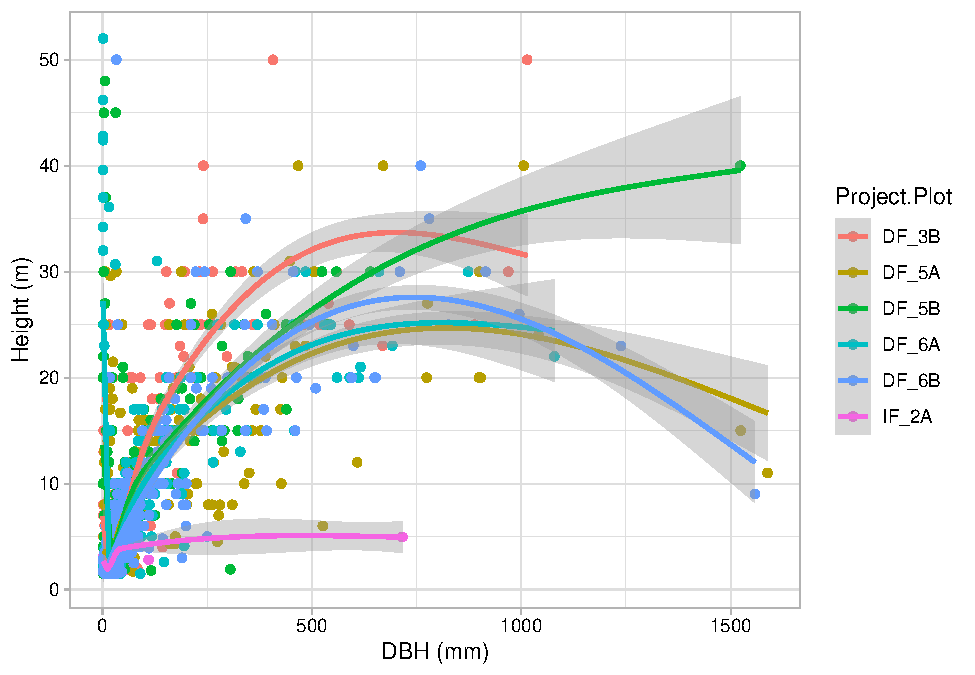
\includegraphics{GoldenGriffithsKnierMalinowski_ENV872_Project_files/figure-latex/plot of DBH vs height-1.pdf}

We added in variables to support our research questions and analyses. We
created two new columns: ``Status'' and ``Distance\_km''

\begin{longtable}[]{@{}llll@{}}
\toprule
\begin{minipage}[b]{0.22\columnwidth}\raggedright
Column name\strut
\end{minipage} & \begin{minipage}[b]{0.32\columnwidth}\raggedright
Description\strut
\end{minipage} & \begin{minipage}[b]{0.17\columnwidth}\raggedright
Unit\strut
\end{minipage} & \begin{minipage}[b]{0.17\columnwidth}\raggedright
Range\strut
\end{minipage}\tabularnewline
\midrule
\endhead
\begin{minipage}[t]{0.22\columnwidth}\raggedright
Status\strut
\end{minipage} & \begin{minipage}[t]{0.32\columnwidth}\raggedright
Indicates whether each plot is defaunated or intact forest\strut
\end{minipage} & \begin{minipage}[t]{0.17\columnwidth}\raggedright
Category\strut
\end{minipage} & \begin{minipage}[t]{0.17\columnwidth}\raggedright
Defaunated - Intact\strut
\end{minipage}\tabularnewline
\begin{minipage}[t]{0.22\columnwidth}\raggedright
Distance\_km\strut
\end{minipage} & \begin{minipage}[t]{0.32\columnwidth}\raggedright
Distance of each plot from Mokokou\strut
\end{minipage} & \begin{minipage}[t]{0.17\columnwidth}\raggedright
Kilometers\strut
\end{minipage} & \begin{minipage}[t]{0.17\columnwidth}\raggedright
8.177 - 40.224\strut
\end{minipage}\tabularnewline
\bottomrule
\end{longtable}

The categorical variable, ``Status'', will help with data visualization,
and the ``Distance\_km'' variable will be used as a proxy from the
defaunation gradient in our analyses.

The new dimensions of this dataset are:

\begin{verbatim}
## [1] 6479    8
\end{verbatim}

Our cleaned dataset looks as follows:

\begin{verbatim}
##   Project.Plot Plant_tag DBH_mm Height_m Veg_Type                     ID
## 1        DF_3B      1554  558.8     30.0     Tree   Heisteria parvifolia
## 2        DF_3B        69   15.8      2.4     Tree   Dialium pachyphyllum
## 3        DF_3B      4371   11.7      1.8  Sapling Scorodophloeus zenkeri
## 4        DF_3B       607   19.4      2.5     Tree    Odjendja gabonensis
## 5        DF_3B      7150   21.5      3.7     Tree Scorodophloeus zenkeri
## 6        DF_3B      7110   65.0      7.5     Tree Centroplacus glaucinus
##       Status Distance_km
## 1 Defaunated      20.195
## 2 Defaunated      20.195
## 3 Defaunated      20.195
## 4 Defaunated      20.195
## 5 Defaunated      20.195
## 6 Defaunated      20.195
\end{verbatim}

Accidental misspellings are common in datasets such as this with
thousands of manual entries of complex Latin species names. This is a
concern because two samples that are supposed to be the same species,
but have different spellings, will not be identified as the same species
in our analyses. By looking at a list of the unique species names in the
dataset, we found this to be the case in several instances. Identifying
these errors and correcting them was very labor intensive as this can
only really be done with the human eye using personal judgment as to
what names were meant to be the same. Before cleaning the species names,
there were 349 ``species''; after correcting for spelling mistakes,
there were only 323 species. This means that 26 ``species'' were falsely
identified prior to data cleaning.

The dimensions of the processed, clean dataset are as follows:

\begin{verbatim}
## [1] 6340    7
\end{verbatim}

\newpage

\hypertarget{exploratory-analysis}{%
\section{Exploratory Analysis}\label{exploratory-analysis}}

\newpage

\hypertarget{spatial-analysis}{%
\subsection{Spatial Analysis}\label{spatial-analysis}}

\hypertarget{dbh}{%
\subsection{DBH}\label{dbh}}

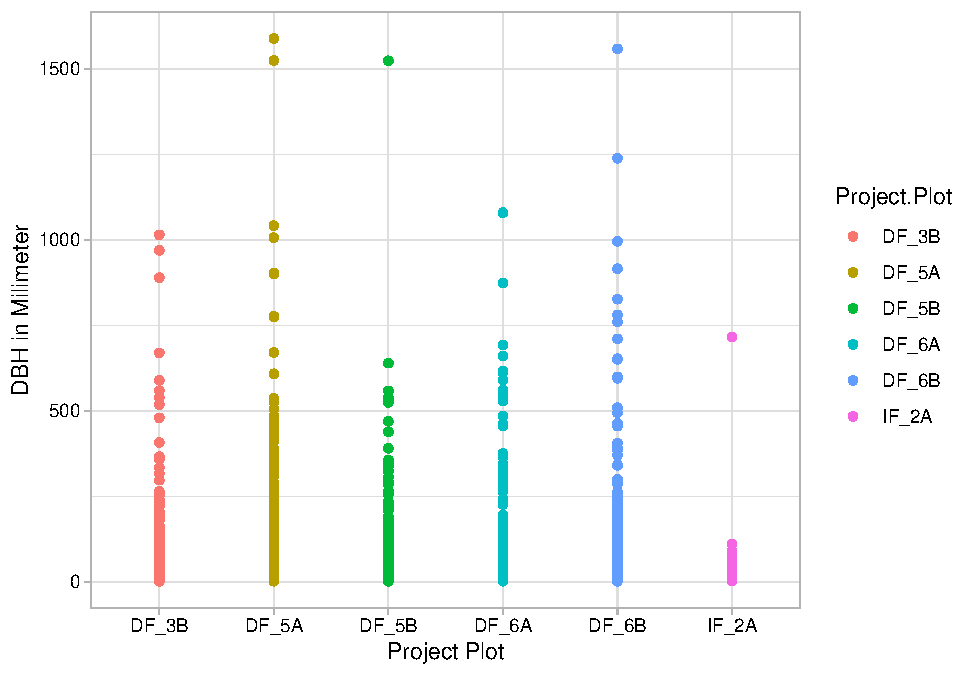
\includegraphics{GoldenGriffithsKnierMalinowski_ENV872_Project_files/figure-latex/DBH graphs-1.pdf}
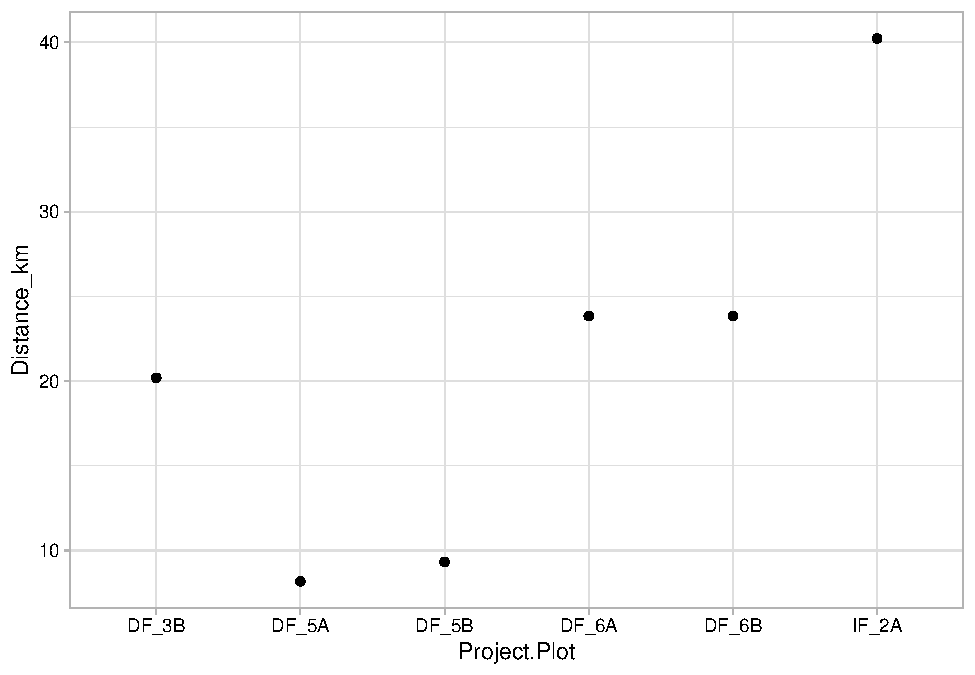
\includegraphics{GoldenGriffithsKnierMalinowski_ENV872_Project_files/figure-latex/DBH graphs-2.pdf}

\begin{verbatim}
## `stat_bin()` using `bins = 30`. Pick better value with `binwidth`.
\end{verbatim}

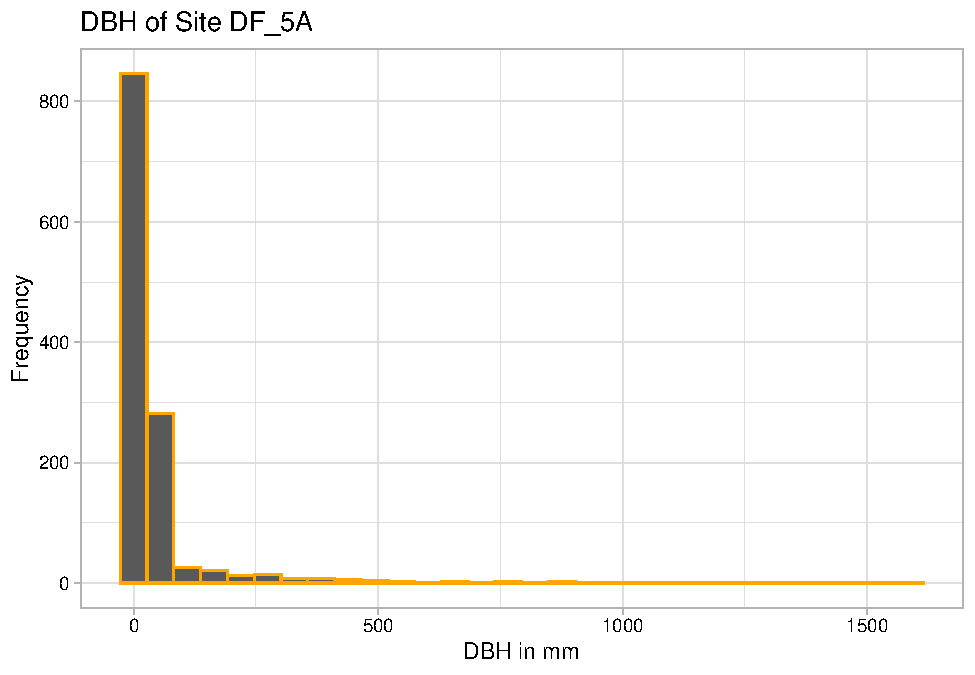
\includegraphics{GoldenGriffithsKnierMalinowski_ENV872_Project_files/figure-latex/DBH graphs-3.pdf}

\begin{verbatim}
## `stat_bin()` using `bins = 30`. Pick better value with `binwidth`.
\end{verbatim}

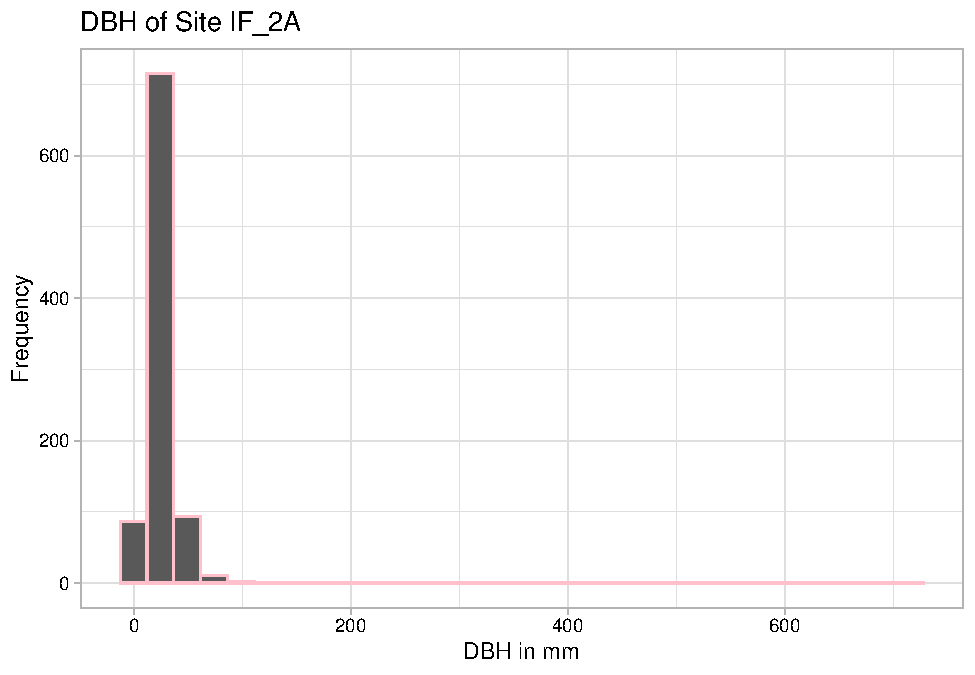
\includegraphics{GoldenGriffithsKnierMalinowski_ENV872_Project_files/figure-latex/DBH graphs-4.pdf}

\begin{verbatim}
## `stat_bin()` using `bins = 30`. Pick better value with `binwidth`.
\end{verbatim}

\begin{verbatim}
## Warning: Removed 12 rows containing non-finite values (stat_bin).
\end{verbatim}

\begin{verbatim}
## Warning: Removed 2 rows containing missing values (geom_bar).
\end{verbatim}

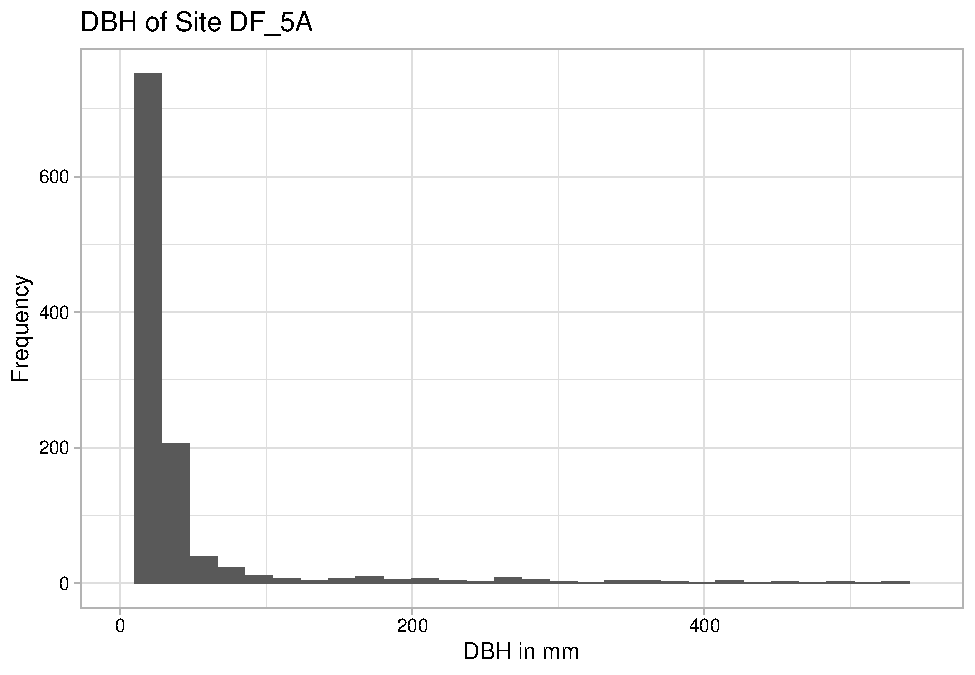
\includegraphics{GoldenGriffithsKnierMalinowski_ENV872_Project_files/figure-latex/DBH graphs-5.pdf}

\begin{verbatim}
## `stat_bin()` using `bins = 30`. Pick better value with `binwidth`.
\end{verbatim}

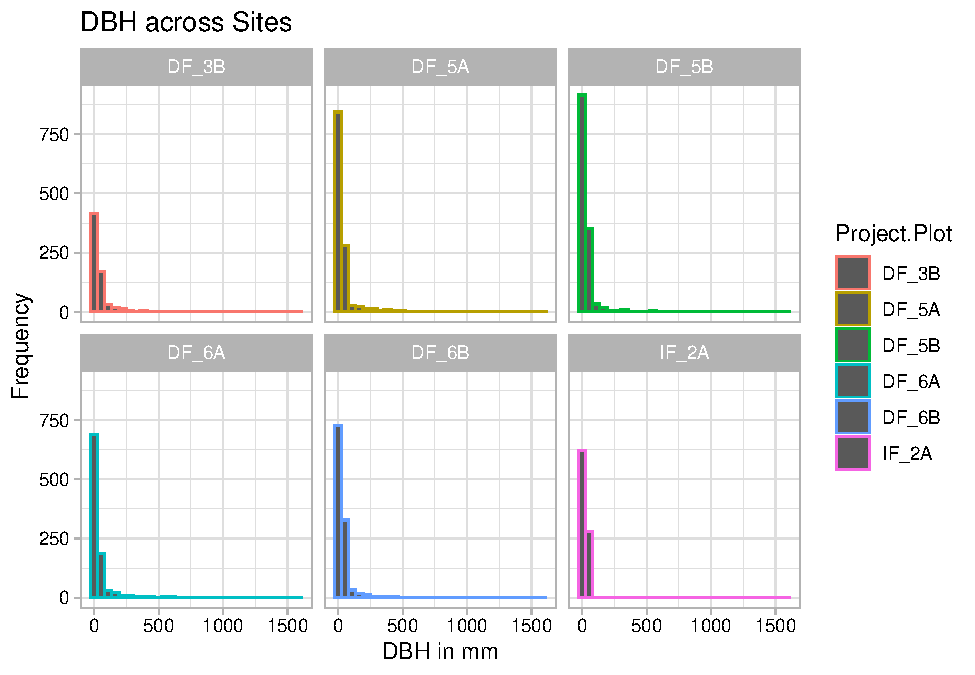
\includegraphics{GoldenGriffithsKnierMalinowski_ENV872_Project_files/figure-latex/DBH graphs-6.pdf}

\begin{verbatim}
## `stat_bin()` using `bins = 30`. Pick better value with `binwidth`.
\end{verbatim}

\begin{verbatim}
## Warning: Removed 284 rows containing non-finite values (stat_bin).
\end{verbatim}

\begin{verbatim}
## Warning: Removed 12 rows containing missing values (geom_bar).
\end{verbatim}

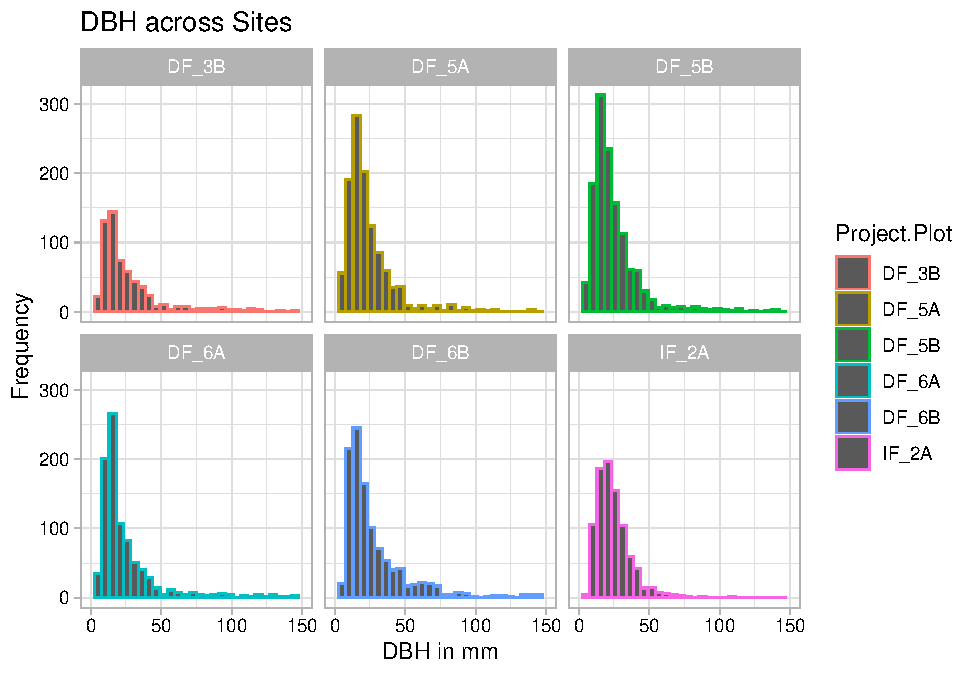
\includegraphics{GoldenGriffithsKnierMalinowski_ENV872_Project_files/figure-latex/DBH graphs-7.pdf}

\begin{verbatim}
## `stat_bin()` using `bins = 30`. Pick better value with `binwidth`.
\end{verbatim}

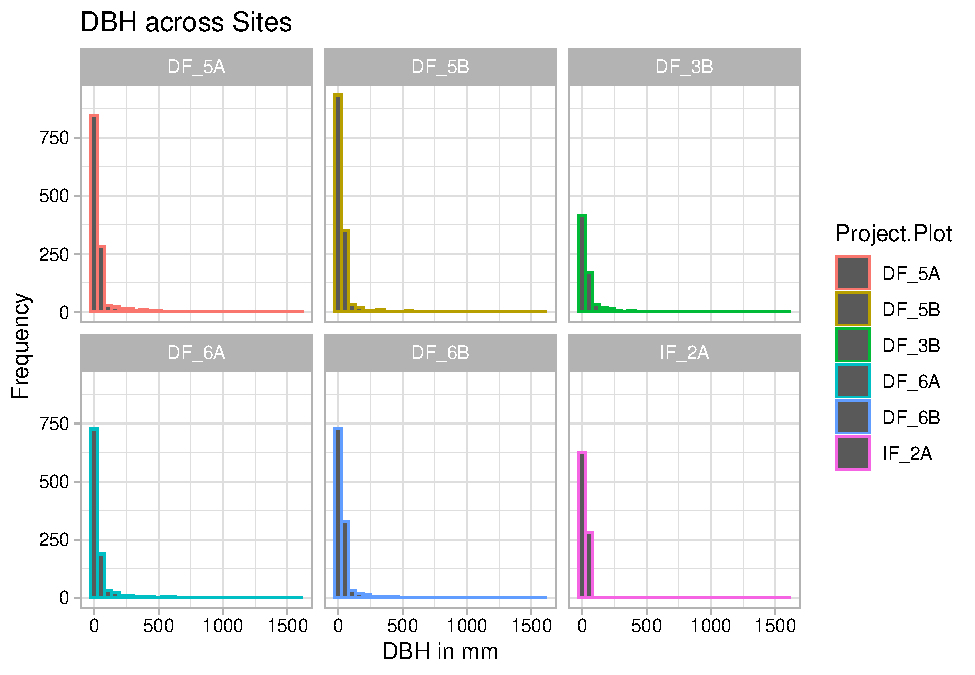
\includegraphics{GoldenGriffithsKnierMalinowski_ENV872_Project_files/figure-latex/DBH graphs-8.pdf}

\begin{verbatim}
## `stat_bin()` using `bins = 30`. Pick better value with `binwidth`.
\end{verbatim}

\begin{verbatim}
## Warning: Removed 284 rows containing non-finite values (stat_bin).

## Warning: Removed 12 rows containing missing values (geom_bar).
\end{verbatim}

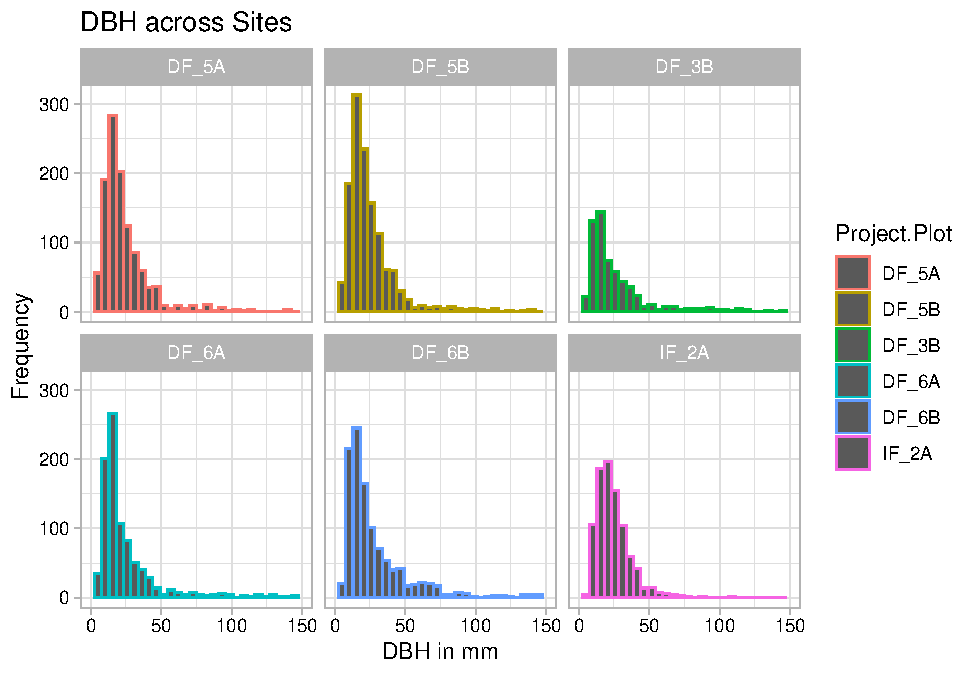
\includegraphics{GoldenGriffithsKnierMalinowski_ENV872_Project_files/figure-latex/DBH graphs-9.pdf}

\begin{verbatim}
##    Min. 1st Qu.  Median    Mean 3rd Qu.    Max. 
##    0.39   14.00   20.15   48.09   32.02 1588.00
\end{verbatim}

\begin{verbatim}
##    Min. 1st Qu.  Median    Mean 3rd Qu.    Max. 
##    0.40   16.00   22.20   25.09   29.80  716.00
\end{verbatim}

\begin{verbatim}
## Warning: Removed 53 rows containing non-finite values (stat_count).
\end{verbatim}

\begin{verbatim}
## Warning: position_stack requires non-overlapping x intervals
\end{verbatim}

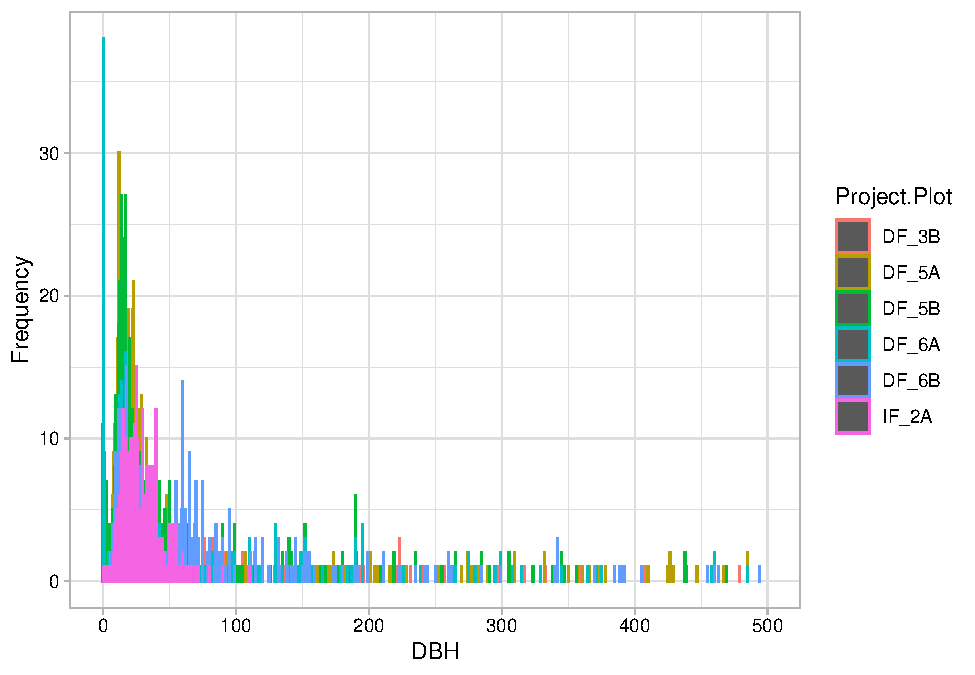
\includegraphics{GoldenGriffithsKnierMalinowski_ENV872_Project_files/figure-latex/DBH graphs-10.pdf}

\hypertarget{analysis}{%
\section{Analysis}\label{analysis}}

\#\#GLMs

So it seems like most sites are pretty not uniform, and small trees are
over-represented at each location. Let's compare sites to see which site
has the most species.

So from this we can see that there are no great disparities between
sites when it comes to species. At 146, DF\_6B has the most species and
at 96 DF\_5B has the fewest species. Most sites have right around 100.
We can also see how each site compares in terms of basal area - i.e.,
how densely forested each site is. IF\_2A has the lowest basal area
where DF\_5A has the greatest at around 15 square meters per hectare.
Given IF\_2A's high species richness but low basal area, these data seem
to suggest that IF\_2A has many small trees but few large ones. Let's
continue our exploration by seeing which genuses contribute the most to
each site's basal area.

From these graphs we can see which genera make up the majority of basal
area at each site. So how similar are these sites to one another? I
wonder. ANOVA?

Let's begin to see if there is any relationship between basal area,
species richness, and distance to towns (i.e., along the defaunation
gradient)?.

Looking at these graphs, it doesn't appear that there's much of an
obvious relationship between basal area, species richness, and distance
along the defaunation gradient. Still, looks can be deceiving. Let's
feed these data into a linear model to see what relationships can be
statistically proved. We begin by checking for correlations among
variables with a corrplot.

from this it appears that basal area per hectare is negatively
correlated with mean distance at the same time, there appears to be a
weak positive correlation between total species and mean distance. Let's
build a model and see how well these correlations predict basal area and
species richness.

In this linear model we use species richness and distance from developed
area to predict the basal area per hectare of a given site. The null
hypothesis is that there is no relationship between basal area per
hectare, species richness, and distance to town. The alternative
hypothesis is that either both species richness and/or distance to town
will influence basal area per hectare. The results of the model (p =
0.16) indicate that no such significant (p\textless0.05) relationships
exist in this subset of data. However, based on these observations (n =
6), there does appear to be a weak negative relationship (p = 0.09)
between distance to town and basal area per hectare. According to the
model, with every additional kilometer of distance there is an
associated 1.3 square meter decline in basal area of forested land. Once
again, these relationships are not considered significant, which means
the explanatory variables included in this model are not sufficient to
explain observed patterns in stand density along the defaunation
gradient. There is no relationship between distance to town and species
richness (p = 0.74).

\hypertarget{question-1-insert-specific-question-here-and-add-additional-subsections-for-additional-questions-below-if-needed}{%
\subsection{Question 1: \textless insert specific question here and add
additional subsections for additional questions below, if
needed\textgreater{}}\label{question-1-insert-specific-question-here-and-add-additional-subsections-for-additional-questions-below-if-needed}}

\hypertarget{question-2}{%
\subsection{Question 2:}\label{question-2}}

\newpage

\hypertarget{summary-and-conclusions}{%
\section{Summary and Conclusions}\label{summary-and-conclusions}}

\newpage

\hypertarget{references}{%
\section{References}\label{references}}

\textless add references here if relevant, otherwise delete this
section\textgreater{}

\end{document}
